\documentclass[12pt,a4paper]{article}
\usepackage[utf8]{vietnam}
\usepackage{amsmath,amssymb}
\usepackage{tabularx}
\usepackage{tikz}
\usetikzlibrary{calc,angles,quotes,arrows.meta}
\usepackage{xcolor}
\usepackage{enumitem}
\usepackage{fancyhdr}
\usepackage[top=1.2cm, bottom=1.2cm, left=1.5cm, right=1.5cm]{geometry}
\usepackage[dethi]{ex_test}
\SAOPTN{widthSA=2.6,heightSA=0.62}

\setlength{\headheight}{15pt}
\setlength{\parskip}{0pt}

% Dòng kẻ chấm mờ chuẩn viết tay
\newcommand{\dongke}[1]{%
  \begingroup%
  \setlength{\parskip}{0pt}%
  \baselineskip=18.5pt%
  \vspace{1.0mm}%
  \foreach \i in {1,...,#1}{%
    \noindent{\color{gray!60}\dotfill}\par%
  }%
  \vspace{0.6mm}%
  \endgroup%
}

\pagestyle{fancy}
\fancyhf{}
\rhead{\textit{Môn Toán 7 -- Đề số 1}}
\lhead{\textit{Bộ đề ôn tập Giữa học kì I}}
\cfoot{\thepage}

\begin{document}

% --- KHUNG TIÊU ĐỀ ĐỀ THI ---
\noindent
\begin{tabularx}{\linewidth}{X r}
\textbf{TRƯỜNG THCS: \dotfill} & \textbf{ĐỀ KIỂM TRA ĐỊNH KỲ GIỮA HỌC KỲ I} \\
\textbf{Họ và tên: \dotfill} & \textbf{NĂM HỌC 2026 -- 2027} \\
\textbf{Lớp: \dotfill \quad SBD: \dotfill} & \textbf{Môn: TOÁN 7} \\
& \textit{Thời gian làm bài: 90 phút (không kể thời gian phát đề)}
\end{tabularx}

\vspace{1.5mm}
\noindent
\begin{tabularx}{\linewidth}{|p{3.5cm}|X|}
\hline
\centering\textbf{Điểm số} & \centering\textbf{Lời nhận xét của thầy cô giáo} \tabularnewline
\rule{0pt}{1.6cm} & \\
\hline
\end{tabularx}

\vspace{2.5mm}
\begin{center}
\textbf{\large ĐỀ SỐ 1}
\end{center}

\noindent\textbf{\large PHẦN I. CÂU TRẮC NGHIỆM NHIỀU PHƯƠNG ÁN LỰA CHỌN (3,0 điểm)}

\textit{Thí sinh trả lời từ câu 1 đến câu 12. Mỗi câu hỏi chỉ chọn một phương án đúng nhất và ghi vào bảng đáp án.}

\vspace{1mm}
\begin{ex}
Kết quả của phép tính $\left(\frac{1}{3}\right)^9 : \left(\frac{1}{3}\right)^6$ là:
\choice
{$-\frac{1}{3}$}
{\True $\left(\frac{1}{3}\right)^3$}
{$\left(-\frac{1}{3}\right)^3$}
{$\frac{1}{3}$}
\end{ex}

\begin{ex}
Tập hợp các số hữu tỉ kí hiệu là:
\choice
{\True $\mathbb{Q}$}
{$\mathbb{N}^*$}
{$\mathbb{N}$}
{$\mathbb{Z}$}
\end{ex}

\begin{ex}
Khẳng định nào sau đây là đúng?
\choice
{Nếu $a$ là số tự nhiên thì $a$ là số vô tỉ}
{\True Nếu $a$ là số hữu tỉ thì $a$ không thể là số vô tỉ}
{Số thập phân vô hạn tuần hoàn là số vô tỉ}
{Số thập phân hữu hạn là số vô tỉ}
\end{ex}

\begin{ex}
\immini{
Đọc tên các tia phân giác trong hình vẽ sau.
\choice
{$AB, BE$ là các tia phân giác}
{$AD, BC$ là các tia phân giác}
{\True $AD, BE$ là các tia phân giác}
{$AD, AB$ là các tia phân giác}
}{
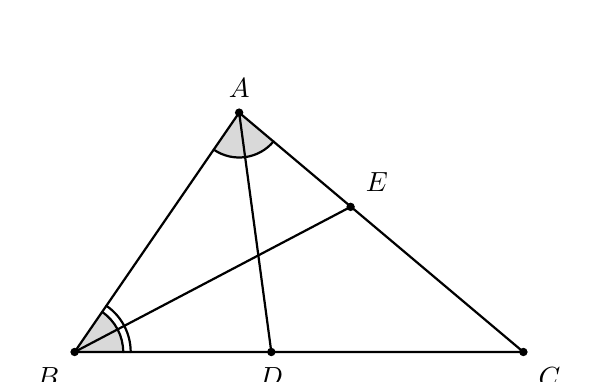
\begin{tikzpicture}[scale=0.95, line cap=round, line join=round]
  \coordinate (B) at (0,0);
  \coordinate (C) at (6,0);
  \coordinate (A) at (2.2,3.2);
  \coordinate (D) at (2.63,0);
  \coordinate (E) at (3.69,1.94);

  % Cung góc A (tô xám nhạt và vẽ cung đơn)
  \fill[gray!30] (A) -- ($(A)!0.6cm!(B)$) arc[start angle=235.5, end angle=320, radius=0.6cm] -- cycle;
  \draw[thick] ($(A)!0.6cm!(B)$) arc[start angle=235.5, end angle=320, radius=0.6cm];

  % Cung góc B (tô xám nhạt và vẽ 2 cung đôi)
  \fill[gray!30] (B) -- (0.65,0) arc[start angle=0, end angle=55.5, radius=0.65cm] -- cycle;
  \draw[thick] (0.65,0) arc[start angle=0, end angle=55.5, radius=0.65cm];
  \draw[thick] (0.75,0) arc[start angle=0, end angle=55.5, radius=0.75cm];

  % Các cạnh tam giác
  \draw[thick] (A) -- (B) -- (C) -- cycle;
  % Hai tia phân giác AD và BE
  \draw[thick] (A) -- (D);
  \draw[thick] (B) -- (E);

  % Các điểm
  \foreach \p in {A,B,C,D,E} \fill (\p) circle (1.6pt);
  \node[above=2pt] at (A) {$A$};
  \node[below left=2pt] at (B) {$B$};
  \node[below right=2pt] at (C) {$C$};
  \node[below=2pt] at (D) {$D$};
  \node[above right=2pt] at (E) {$E$};
\end{tikzpicture}
}
\end{ex}

\begin{ex}
\immini{
Cho $a//b$, số đo góc $x$ trên hình vẽ bằng:
\choice
{\True $115^\circ$}
{$90^\circ$}
{$65^\circ$}
{$0^\circ$}
}{
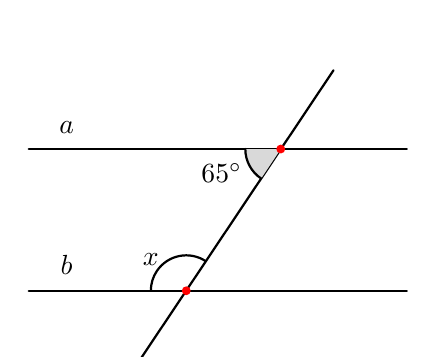
\begin{tikzpicture}[scale=1.0, line cap=round, line join=round]
  \coordinate (B) at (1.8,0);
  \coordinate (A) at (3.0,1.8);

  % Hai đường thẳng song song a và b
  \draw[thick] (-0.2,1.8) -- (4.6,1.8) node[above=2pt, pos=0.1] {$a$};
  \draw[thick] (-0.2,0)   -- (4.6,0)   node[above=2pt, pos=0.1] {$b$};

  % Cát tuyến cắt a tại A, b tại B
  \draw[thick] (1.13,-1.0) -- (3.67,2.8);

  % Góc 65° tại A: trong cùng phía (dưới a, bên trái cát tuyến)
  \fill[gray!30] (A) -- ++(180:0.45) arc[start angle=180, end angle=236.3, radius=0.45] -- cycle;
  \draw[thick] (A) ++(180:0.45) arc[start angle=180, end angle=236.3, radius=0.45];
  \node at ($(A)+(-0.75,-0.3)$) {$65^\circ$};

  % Góc tù x tại B: trong cùng phía (trên b, bên trái cát tuyến)
  \draw[thick] (B) ++(56.3:0.45) arc[start angle=56.3, end angle=180, radius=0.45];
  \node at ($(B)+(-0.45,0.4)$) {$x$};

  % Giao điểm đỏ
  \fill[red] (A) circle (1.6pt);
  \fill[red] (B) circle (1.6pt);
\end{tikzpicture}
}
\end{ex}

\begin{ex}
Chọn đáp án sai. Hai góc đối đỉnh là
\choice
{Hai góc bằng nhau}
{Hai góc mà mỗi cạnh của góc này là tia đối của một cạnh của góc kia}
{\True Hai góc có tổng số đo bằng $180^0$}
{Hai góc được tạo bởi hai đường thẳng cắt nhau}
\end{ex}

\begin{ex}
Cho trục số sau: Điểm $A$ biểu diễn số nào trên trục số?
\begin{center}
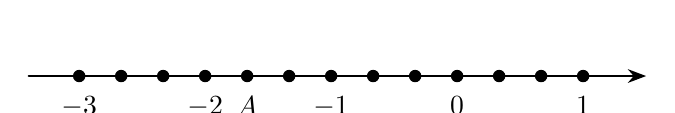
\begin{tikzpicture}[scale=1.6, line cap=round, line join=round, >=Stealth]
  % Trục số có mũi tên sang phải
  \draw[thick, ->] (-3.4,0) -- (1.5,0);
  % Các chấm chia 1/3 đơn vị
  \foreach \i in {-9,-8,...,3}{
    \fill ({\i/3},0) circle (1.4pt);
  }
  % Nhãn các số nguyên chính
  \node[below=4pt] at (-3,0) {$-3$};
  \node[below=4pt] at (-2,0) {$-2$};
  \node[below=4pt] at (-1,0) {$-1$};
  \node[below=4pt] at (0,0)  {$0$};
  \node[below=4pt] at (1,0)  {$1$};

  % Điểm A tại -5/3 = -1 2/3
  \node[below=4pt, font=\bfseries] at (-5/3,0) {$A$};
\end{tikzpicture}
\end{center}
\choice
{$-2\frac{1}{3}$}
{$-1\frac{1}{3}$}
{\True $-1\frac{2}{3}$}
{$-2\frac{2}{3}$}
\end{ex}

\begin{ex}
Cho $a//b$ và $b//c$, khi đó:
\choice
{$a \perp c$}
{\True $a // c$}
{$c \perp b$}
{$a \perp b$}
\end{ex}

\begin{ex}
Căn bậc hai số học của $81$ là
\choice
{\True $9$}
{$-9$}
{$9$ và $-9$}
{$81$}
\end{ex}

\begin{ex}
Trong các hình sau, hình nào là hình lăng trụ đứng tam giác?
\begin{center}
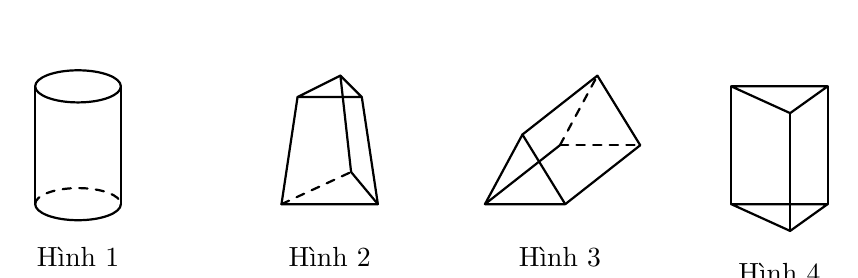
\begin{tikzpicture}[scale=0.68, line cap=round, line join=round, thick]
  % Hình 1: Hình trụ
  \begin{scope}[shift={(0,0)}]
    \draw (0,2.2) ellipse (0.8 and 0.3);
    \draw (-0.8,0) -- (-0.8,2.2);
    \draw (0.8,0) -- (0.8,2.2);
    \draw (-0.8,0) arc[start angle=180, end angle=360, x radius=0.8, y radius=0.3];
    \draw[dashed] (-0.8,0) arc[start angle=180, end angle=0, x radius=0.8, y radius=0.3];
    \node[below=4pt] at (0,-0.4) {Hình 1};
  \end{scope}

  % Hình 2: Hình chóp cụt tam giác
  \begin{scope}[shift={(3.8,0)}]
    \draw (0,0) -- (1.8,0) -- (1.3,0.6);
    \draw (0.3,2.0) -- (1.5,2.0) -- (1.1,2.4) -- cycle;
    \draw (0,0) -- (0.3,2.0);
    \draw (1.8,0) -- (1.5,2.0);
    \draw (1.3,0.6) -- (1.1,2.4);
    \draw[dashed] (0,0) -- (1.3,0.6);
    \node[below=4pt] at (0.9,-0.4) {Hình 2};
  \end{scope}

  % Hình 3: Lăng trụ tam giác nằm ngang
  \begin{scope}[shift={(7.6,0)}]
    \draw (0,0) -- (1.5,0) -- (0.7,1.3) -- cycle;
    \draw (0.7,1.3) -- (2.1,2.4);
    \draw (1.5,0) -- (2.9,1.1);
    \draw (2.1,2.4) -- (2.9,1.1);
    \draw (0,0) -- (1.4,1.1);
    \draw[dashed] (1.4,1.1) -- (2.1,2.4);
    \draw[dashed] (1.4,1.1) -- (2.9,1.1);
    \node[below=4pt] at (1.4,-0.4) {Hình 3};
  \end{scope}

  % Hình 4: Lăng trụ đứng tam giác
  \begin{scope}[shift={(12.2,0)}]
    \draw (0,2.2) -- (1.8,2.2) -- (1.1,1.7) -- cycle;
    \draw (0,0) -- (1.8,0) -- (1.1,-0.5) -- cycle;
    \draw (0,0) -- (0,2.2);
    \draw (1.8,0) -- (1.8,2.2);
    \draw (1.1,-0.5) -- (1.1,1.7);
    \node[below=4pt] at (0.9,-0.7) {Hình 4};
  \end{scope}
\end{tikzpicture}
\end{center}
\choice
{Hình 1}
{Hình 2}
{Hình 3}
{\True Hình 4}
\end{ex}

\begin{ex}
Trong các hình sau, hình nào không phải là hình lăng trụ đứng tứ giác?
\begin{center}
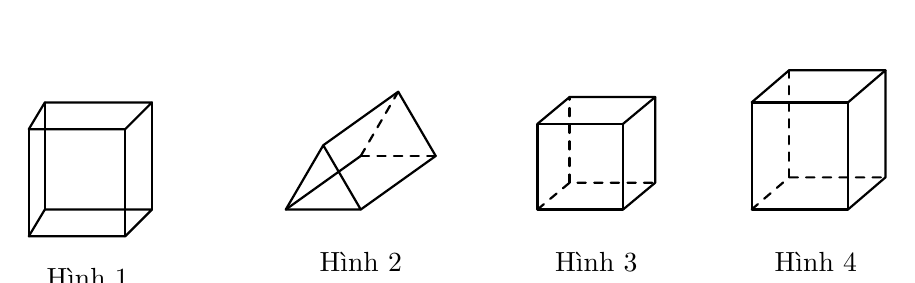
\begin{tikzpicture}[scale=0.68, line cap=round, line join=round, thick]
  % Hình 1: Lăng trụ tứ giác
  \begin{scope}[shift={(0,0)}]
    \draw (0,0) -- (2.0,0) -- (1.5,-0.5) -- (-0.3,-0.5) -- cycle;
    \draw (0,2.0) -- (2.0,2.0) -- (1.5,1.5) -- (-0.3,1.5) -- cycle;
    \draw (0,0) -- (0,2.0);
    \draw (2.0,0) -- (2.0,2.0);
    \draw (1.5,-0.5) -- (1.5,1.5);
    \draw (-0.3,-0.5) -- (-0.3,1.5);
    \node[below=4pt] at (0.8,-0.7) {Hình 1};
  \end{scope}

  % Hình 2: Lăng trụ tam giác nằm ngang (đáp án đúng)
  \begin{scope}[shift={(4.5,0)}]
    \draw (0,0) -- (1.4,0) -- (0.7,1.2) -- cycle;
    \draw (0,0) -- (1.4,1.0);
    \draw (0.7,1.2) -- (2.1,2.2);
    \draw (1.4,0) -- (2.8,1.0);
    \draw (2.1,2.2) -- (2.8,1.0);
    \draw[dashed] (1.4,1.0) -- (2.1,2.2);
    \draw[dashed] (1.4,1.0) -- (2.8,1.0);
    \node[below=4pt] at (1.4,-0.4) {Hình 2};
  \end{scope}

  % Hình 3: Hình lập phương
  \begin{scope}[shift={(9.2,0)}]
    \draw (0,0) rectangle (1.6,1.6);
    \draw (1.6,0) -- (2.2,0.5) -- (2.2,2.1) -- (1.6,1.6);
    \draw (0,1.6) -- (0.6,2.1) -- (2.2,2.1);
    \draw[dashed] (0,0) -- (0.6,0.5) -- (2.2,0.5);
    \draw[dashed] (0.6,0.5) -- (0.6,2.1);
    \node[below=4pt] at (1.1,-0.4) {Hình 3};
  \end{scope}

  % Hình 4: Lăng trụ tứ giác đứng
  \begin{scope}[shift={(13.2,0)}]
    \draw (0,0) rectangle (1.8,2.0);
    \draw (1.8,0) -- (2.5,0.6) -- (2.5,2.6) -- (1.8,2.0);
    \draw (0,2.0) -- (0.7,2.6) -- (2.5,2.6);
    \draw[dashed] (0,0) -- (0.7,0.6) -- (2.5,0.6);
    \draw[dashed] (0.7,0.6) -- (0.7,2.6);
    \node[below=4pt] at (1.2,-0.4) {Hình 4};
  \end{scope}
\end{tikzpicture}
\end{center}
\choice
{Hình 1}
{\True Hình 2}
{Hình 3}
{Hình 4}
\end{ex}

\begin{ex}
Trong các số sau, số nào là số vô tỉ?
\choice
{$-7$}
{$4,2$}
{\True $\sqrt{11}$}
{$\frac{5}{3}$}
\end{ex}


\vspace{1mm}
\noindent\textbf{BẢNG TRẢ LỜI TRẮC NGHIỆM PHẦN I:}
\begin{center}
\begin{tabular}{|c|c|c|c|c|c|c|c|c|c|c|c|c|}
\hline
\textbf{Câu} & \textbf{1} & \textbf{2} & \textbf{3} & \textbf{4} & \textbf{5} & \textbf{6} & \textbf{7} & \textbf{8} & \textbf{9} & \textbf{10} & \textbf{11} & \textbf{12} \\
\hline
\textbf{Chọn} & \rule{0pt}{0.65cm} & & & & & & & & & & & \\
\hline
\end{tabular}
\end{center}
\vspace{2mm}

\setcounter{ex}{0}
\noindent\textbf{\large PHẦN II. CÂU TRẮC NGHIỆM ĐÚNG SAI (2,0 điểm)}

\textit{Thí sinh trả lời câu 1 và câu 2. Trong mỗi ý a), b), c), d) ở mỗi câu, thí sinh chọn đúng hoặc sai.}

\vspace{1mm}
\begin{ex}
Cho các số: $0,15$; $-2,(4)$; $\dfrac{2}{3}$; $1,02(5)$; $0,(21)$; $-0,0181818$; $\dfrac{3}{10}$. Xét tính đúng sai của các mệnh đề sau:
\choiceTF
{\True Các số $0,15$; $-0,0181818$ là các số thập phân hữu hạn}
{Các số $-2,(4)$; $1,02(5)$; $0,(21)$; $-0,0181818$ là các số thập phân vô hạn tuần hoàn}
{Từ đẳng thức $\dfrac{2}{3}x+\dfrac{7}{10}=\dfrac{3}{10}$ ta suy ra được $\dfrac{2}{3}x=\dfrac{3}{10}+\dfrac{7}{10}$}
{\True Giá trị của $x$ thỏa mãn $\dfrac{2}{3}x+\dfrac{7}{10}=\dfrac{3}{10}$ là $x=\dfrac{-3}{5}$}
\end{ex}

\begin{ex}
\immini{
Cho hình vẽ, biết đường thẳng $a$ vuông góc với $CD$ tại $C$, đường thẳng $b$ vuông góc với $CD$ tại $D$ và góc $\widehat{B_4}=120^\circ$. Xét tính đúng sai của các mệnh đề sau:
\choiceTF
{\True $\widehat{B_2}=120^\circ$}
{\True $\widehat{B_3}=60^\circ$}
{\True $a\parallel b$}
{Góc kề bù với góc $\widehat{A_1}$ bằng $150^\circ$}
}{
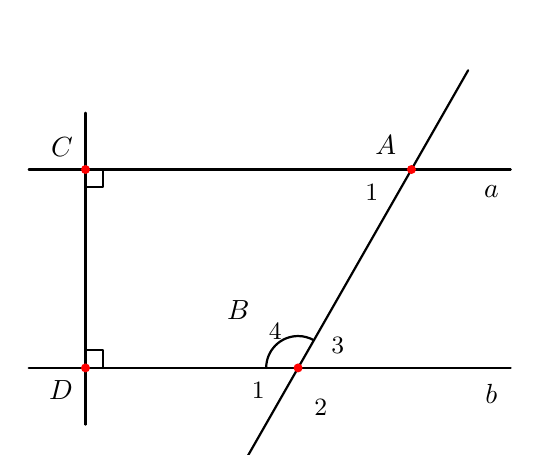
\begin{tikzpicture}[scale=0.9, line cap=round, line join=round]
  \coordinate (C) at (0, 2.8);
  \coordinate (D) at (0, 0);
  \coordinate (B) at (3.0, 0);
  \coordinate (A) at (4.6, 2.8);

  % Đường CD thẳng đứng kéo dài
  \draw[thick] (0, 3.6) -- (0, -0.8);
  % Đường thẳng a qua C, A
  \draw[thick] (-0.8, 2.8) -- (6.0, 2.8) node[below=2pt, pos=0.96] {$a$};
  % Đường thẳng b qua D, B
  \draw[thick] (-0.8, 0)   -- (6.0, 0)   node[below=2pt, pos=0.96] {$b$};

  % Cát tuyến BA kéo dài rõ ràng hai đầu (từ dưới b lên trên a)
  \draw[thick] (2.2, -1.4) -- (5.4, 4.2);

  % Ký hiệu góc vuông tại C và D
  \draw[thick] (0, 2.55) -- (0.25, 2.55) -- (0.25, 2.8);
  \draw[thick] (0, 0.25) -- (0.25, 0.25) -- (0.25, 0);

  % Các giao điểm đỏ
  \foreach \p in {C,D,A,B} \fill[red] (\p) circle (1.8pt);
  \node[above left=1pt] at (C) {$C$};
  \node[below left=1pt] at (D) {$D$};
  \node[above left=2pt] at (A) {$A$};
  \node[above left=14pt] at (B) {$B$};

  % Góc A1
  \node[font=\small] at (4.04, 2.48) {$1$};

  % Cung góc B4 (120°)
  \draw[thick] ($(B)+(-0.45,0)$) arc[start angle=180, end angle=60.3, radius=0.45cm];

  % Các góc 1, 2, 3, 4 tại B (đặt chính xác trong 4 góc phần tư, không đè nhãn B hay vạch kẻ)
  \node[font=\small] at (2.68, 0.52) {$4$};
  \node[font=\small] at (3.56, 0.32) {$3$};
  \node[font=\small] at (2.44, -0.32) {$1$};
  \node[font=\small] at (3.32, -0.56) {$2$};
\end{tikzpicture}
}
\end{ex}


\noindent\textbf{BẢNG TRẢ LỜI PHẦN II:}
\begin{center}
\begin{tabular}{|c|c|c|c|c||c|c|c|c|c|}
\hline
\textbf{Câu 1} & \textbf{a)} & \textbf{b)} & \textbf{c)} & \textbf{d)} & \textbf{Câu 2} & \textbf{a)} & \textbf{b)} & \textbf{c)} & \textbf{d)} \\
\hline
\textbf{Đ/S} & \rule{0pt}{0.6cm} & & & & \textbf{Đ/S} & & & & \\
\hline
\end{tabular}
\end{center}
\vspace{2mm}

\setcounter{ex}{0}
\noindent\textbf{\large PHẦN III. CÂU HỎI TRẢ LỜI NGẮN (1,0 điểm)}

\textit{Thí sinh trả lời câu 1 và câu 2. Điền kết quả vào ô trống.}

\vspace{1mm}
\begin{ex}
Cho $\widehat{xOy}=70^\circ$, $Ot$ là tia phân giác của $\widehat{xOy}$. Số đo $\widehat{xOt}$ bằng bao nhiêu? \shortans{35^\circ}
\end{ex}

\begin{ex}
Tìm giá trị của $x$, biết: $\dfrac{1}{4}-\dfrac{5}{2}x=\dfrac{3}{2}$ (kết quả ghi dưới dạng số thập phân). \shortans{-0.5}
\end{ex}


\setcounter{ex}{0}
\noindent\textbf{\large PHẦN IV. TỰ LUẬN (4,0 điểm)}

\textit{Thí sinh trình bày chi tiết lời giải vào giấy làm bài.}

\vspace{1mm}
\begin{ex}
Tính hợp lí
\begin{enumerate}[label=\textbf{\alph*)}, leftmargin=0.8cm, itemsep=1pt]
\item $\dfrac{3}{5}\cdot\dfrac{7}{9}+\dfrac{3}{5}\cdot\dfrac{2}{9}$
\item $\left(2025+\dfrac{1}{2}+\dfrac{3}{7}\right)-\left(\dfrac{1}{2}+2025+\dfrac{3}{7}\right)$
\end{enumerate}
\end{ex}
\vspace{1.5mm}

\begin{ex}
Tìm $x$, biết:
\begin{enumerate}[label=\textbf{\alph*)}, leftmargin=0.8cm, itemsep=1pt]
\item $2\dfrac{1}{4}x-4=\dfrac{1}{2}$
\item $\dfrac{x-1}{4}=\dfrac{-1}{2}$
\item $2.(x-1)^2=3^3+5$
\end{enumerate}
\end{ex}
\vspace{1.5mm}

\begin{ex}
\immini{
Cho hình vẽ, biết $a\perp AB$; $b\perp AB$; $\widehat{C}=100^\circ$.
\begin{enumerate}[label=\textbf{\alph*)}, leftmargin=0.8cm, itemsep=1pt]
\item Chứng tỏ $a\parallel b$.
\item Tính $\widehat{D_1}$.
\end{enumerate}
}{
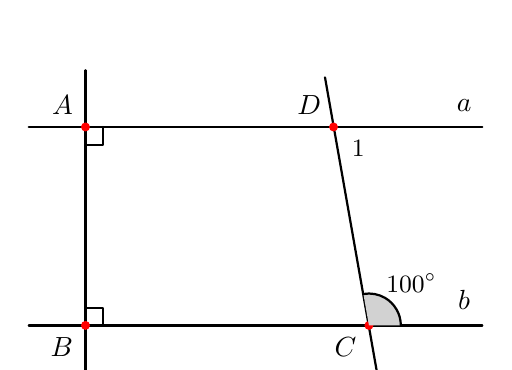
\begin{tikzpicture}[scale=0.9, line cap=round, line join=round]
  \coordinate (A) at (0, 2.8);
  \coordinate (B) at (0, 0);
  \coordinate (D) at (3.5, 2.8);
  \coordinate (C) at (4.0, 0);

  % Đoạn AB thẳng đứng kéo dài
  \draw[thick] (0, 3.6) -- (0, -0.8);
  % Đường a qua A, D
  \draw[thick] (-0.8, 2.8) -- (5.6, 2.8) node[above=2pt, pos=0.96] {$a$};
  % Đường b qua B, C
  \draw[thick] (-0.8, 0)   -- (5.6, 0)   node[above=2pt, pos=0.96] {$b$};

  % Cát tuyến CD kéo dài rõ ràng hai đầu (từ dưới b lên trên a)
  \draw[thick] (4.12, -0.7) -- (3.38, 3.5);

  % Ký hiệu góc vuông tại A và B
  \draw[thick] (0, 2.55) -- (0.25, 2.55) -- (0.25, 2.8);
  \draw[thick] (0, 0.25) -- (0.25, 0.25) -- (0.25, 0);

  % Các giao điểm đỏ
  \foreach \p in {A,B,C,D} \fill[red] (\p) circle (1.8pt);
  \node[above left=1pt] at (A) {$A$};
  \node[below left=1pt] at (B) {$B$};
  \node[above left=1pt] at (D) {$D$};
  \node[below left=1pt] at (C) {$C$};

  % Cung góc C = 100° (tô xám nhẹ)
  \fill[gray!35] (C) -- ++(0:0.45) arc[start angle=0, end angle=100, radius=0.45] -- cycle;
  \draw[thick] (C) ++(0:0.45) arc[start angle=0, end angle=100, radius=0.45];
  \node[font=\small] at ($(C)+(45:0.85)$) {$100^\circ$};

  % Nhãn góc D1
  \node[font=\small] at (3.85, 2.5) {$1$};
\end{tikzpicture}
}
\end{ex}
\vspace{1.5mm}

\begin{ex}
Tính các góc của tam giác $ABC$ biết: $\dfrac{\widehat{A}}{3}=\dfrac{\widehat{B}}{4}=\dfrac{\widehat{C}}{2}$.
\end{ex}
\vspace{1.5mm}


\begin{center}
\rule{4cm}{0.4pt}\\
\textit{--- HẾT ---}
\end{center}
\end{document}
